\documentclass[12pt, titlepage]{article}

\usepackage{fullpage}
\usepackage[round]{natbib}
\usepackage{multirow}
\usepackage{booktabs}
\usepackage{tabularx}
\usepackage{graphicx}
\usepackage{float}
\usepackage{hyperref}
\usepackage[normalem]{ulem}

\hypersetup{
    colorlinks,
    citecolor=black,
    filecolor=black,
    linkcolor=red,
    urlcolor=blue
}
\usepackage[round]{natbib}

\newcounter{acnum}
\newcommand{\actheacnum}{AC\theacnum}
\newcommand{\acref}[1]{AC\ref{#1}}

\newcounter{ucnum}
\newcommand{\uctheucnum}{UC\theucnum}
\newcommand{\uref}[1]{UC\ref{#1}}

\newcounter{mnum}
\newcommand{\mthemnum}{M\themnum}
\newcommand{\mref}[1]{M\ref{#1}}

\title{SE 3XA3: Module Guide\\T-Rex Acceleration}

\author{Team 15, Dev\textsuperscript{enthusiasts}
		\\ Zihao Du (duz12)
		\\ Andrew Balmakund (balmakua) 
		\\ Namit Chopra (choprn9)
}


\date{\today}


\begin{document}

\maketitle

\pagenumbering{roman}
\tableofcontents
\listoftables
\listoffigures

\begin{table}[bp]
\caption{\bf Revision History}
\begin{tabularx}{\textwidth}{p{3cm}p{2cm}X}
\toprule {\bf Date} & {\bf Version} & {\bf Notes}\\
\midrule
03/18/2021 & 1.0 & Initial Version\\
\textcolor{red}{04/07/2021} & \textcolor{red}{2.0} & \textcolor{red}{Revision 1}\\
\bottomrule
\end{tabularx}
\end{table}

\newpage

\pagenumbering{arabic}

\section{Introduction}
\subsection*{Overview}
T-Rex Acceleration is a python based implementation of the Google Chrome game T-Rex Runner, which is implemented with JavaScript. The goal of the project is to create a new version of T-Rex Runner game based on the existing implementation with a fresh twist. New features like changing volume and powerups will be added to the project. This project also uses the MVC design pattern to design all modules.
\subsection*{Context}
The module guide (MG) is based on the functional and non-functional requirements mentioned in the software requirements specification (SRS). The purpose of the document is to provide developers with a modular structure of the system, and how requirements can be met and traced in the structure. It is also helpful to check the interaction between modules and the consistency of the system. Along with MG, there will be a module interface specification (MIS) document in which these modules are specified in detail, including access routine, state variable, etc.
\subsection*{Design Principles}
We advocate a decomposition based on the principle of information hiding~\citep{Parnas1972a}. This
principle supports design for change because of the ``secrets'' that each module hides represent likely future changes. Design for change is valuable in software development, where modifications are frequent, especially during initial development as the solution space is explored.  
\subsection*{Document Structure}
The rest of the document is organized as follows. Section
\ref{SecChange} lists the anticipated and unlikely changes of the software
requirements. Section \ref{SecMH} summarizes the module decomposition that
was constructed according to the likely changes. Section \ref{SecConnection}
specifies the connections between the software requirements and the
modules. Section \ref{SecMD} gives a detailed description of the
modules. Section \ref{SecTM} includes two traceability matrices. One checks
the completeness of the design against the requirements provided in the SRS. The
other shows the relation between anticipated changes and the modules. Section
\ref{SecUse} describes the use relation between modules.
\section{Anticipated and Unlikely Changes}
\label{SecChange}

This section lists possible changes to the system. According to the likeliness
of the change, the possible changes are classified into two
categories. Anticipated changes are listed in Section \ref{SecAchange}, and
unlikely changes are listed in Section \ref{SecUchange}.

\subsection{Anticipated Changes} \label{SecAchange}

Anticipated changes are the source of the information that is to be hidden
inside the modules. Ideally, changing one of the anticipated changes will only
require changing the one module that hides the associated decision. The approach
adapted here is called design for
change.

\begin{description}
\item[\refstepcounter{acnum} \actheacnum \label{ac1}:] The method to generate new background colours.
\item[\refstepcounter{acnum} \actheacnum \label{ac2}:] The number and types of powerups that can be acquired by the player.
\item [\refstepcounter{acnum} \actheacnum \label{ac3}:] The number and types of obstacles that the player has to avoid.
\item [\refstepcounter{acnum} \actheacnum \label{ac4}:] New images for the character, powerups, obstacles, and environment.
\item [\refstepcounter{acnum} \actheacnum \label{ac5}:] Sounds files associated with different game features.
\item [\refstepcounter{acnum} \actheacnum \label{ac6}:] The dimensions and position of the character, powerups, obstacles, and environment drawn on the screen.
\end{description}

\subsection{Unlikely Changes} \label{SecUchange}

The module design should be as general as possible. However, a general system is
more complex. Sometimes this complexity is not necessary. Fixing some design
decisions at the system architecture stage can simplify the software design. If
these decision should later need to be changed, then many parts of the design
will potentially need to be modified. Hence, it is not intended that these
decisions will be changed.

\begin{description}
\item[\refstepcounter{ucnum} \uctheucnum \label{ucIO}:] The only way to interact with the system by using the keyboard (except the close button of the window \color{red}{and setting menu}\color{black}{). The user must use the keyboard to control the character during the game. The keyboard is also needed to navigate through the main, pause, and end menu. This includes the settings menu as well, which is accessed through the main menu.}
\item[\refstepcounter{ucnum} \uctheucnum \label{ucInput}:] The number of players, currently one, that can play the game at once on the same machine is not expected to change. The game is designed to be played by one player and that is kept in mind when designing all the modules.
\item[\refstepcounter{ucnum} \uctheucnum \label{ucInput}:] The environment and platforms where the game can be played are unlikely to be changed. The game is expected to be supported by Windows, macOS, and Linux. 
\end{description}


\section{Module Hierarchy} \label{SecMH}

This section provides an overview of the module design. Modules are summarized
in a hierarchy decomposed by secrets in Table \ref{TblMH}. The modules listed
below, which are leaves in the hierarchy tree, are the modules that will
actually be implemented.




\begin{description}
    \item [\refstepcounter{mnum} \mthemnum \label{m1}:] Character
    \item [\refstepcounter{mnum} \mthemnum \label{m2}:] Powerups
    \item [\refstepcounter{mnum} \mthemnum \label{m3}:] Obstacle
    \item [\refstepcounter{mnum} \mthemnum \label{m4}:] DetectCollision
    \item [\refstepcounter{mnum} \mthemnum \label{m5}:] UpdateEnvironment
    \item [\refstepcounter{mnum} \mthemnum \label{m6}:] Score
    \item \sout{[\refstepcounter{mnum} \mthemnum \label{m7}:] MainMenu}
    \item [\refstepcounter{mnum} \mthemnum \label{m8}:] DisplayObstacle
    \item [\refstepcounter{mnum} \mthemnum \label{m9}:] DisplayPowerups
    \item [\refstepcounter{mnum} \mthemnum \label{m10}:] DisplayEnvironment
    \item [\refstepcounter{mnum} \mthemnum \label{m11}:] DisplayWindow
    \item [\refstepcounter{mnum} \mthemnum \label{m12}:] DisplayCharacter
    \item [\refstepcounter{mnum} \mthemnum \label{m13}:] PlaySound
    \item [\refstepcounter{mnum} \mthemnum \label{m14}:] DisplayMenu
    \item [\refstepcounter{mnum} \mthemnum \label{m15}:] LoadAssets
    \item [\refstepcounter{mnum} \mthemnum \label{m16}:] GameController
    \item [\refstepcounter{mnum} \mthemnum \label{m17}:] MenuController

\end{description}

\begin{table}[H]
\centering
\begin{tabular}{p{0.3\textwidth} p{0.6\textwidth}}
\toprule
\textbf{Level 1} & \textbf{Level 2}\\
\midrule

\multirow{7}{0.3\textwidth}{Hardware-Hiding Module} 
    & DisplayMenu\\
& DisplayCharacter\\
    & DisplayPowerups\\
    & DisplayObstacles\\
    & DisplayEnvironment\\
    & PlaySound\\
    & DisplayWindow\\
    & LoadAssets\\
\midrule

\multirow{3}{0.3\textwidth}{Behaviour-Hiding Module} 
& GameController \\
    & MenuController\\
\midrule

\multirow{7}{0.3\textwidth}{Software Decision Module} 
    & Character\\
    & Powerups\\
    & Obstacle\\
    & DetectCollision\\
    & UpdateEnvironment\\
    & Score\\
    & \sout{MainMenu}\\
    
\bottomrule
\end{tabular}
\caption{Module Hierarchy}
\label{TblMH}
\end{table}


\section{Connection Between Requirements and Design} \label{SecConnection}

The design of the system is intended to satisfy the requirements developed in
the SRS. In this stage, the system is decomposed into modules. The connection
between requirements and modules is listed in Table \ref{TblRT}.

\section{Module Decomposition} \label{SecMD}

Modules are decomposed according to the principle of ``information hiding''
proposed by \citet{ParnasEtAl1984}. The \emph{Secrets} field in a module
decomposition is a brief statement of the design decision hidden by the
module. The \emph{Services} field specifies \emph{what} the module will do
without documenting \emph{how} to do it. For each module, a suggestion for the
implementing software is given under the \emph{Implemented By} title. If the
entry is \emph{OS}, this means that the module is provided by the operating
system or by standard programming language libraries.  Also indicate if the
module will be implemented specifically for the software.

Only the leaf modules in the
hierarchy have to be implemented. If a dash (\emph{--}) is shown, this means
that the module is not a leaf and will not have to be implemented. Whether or
not this module is implemented depends on the programming language
selected.

\subsection{Hardware Hiding Modules}
\begin{description}
\item[Secrets:]The data structure and algorithm used to implement the virtual
  hardware.
\item[Services:]Serve as a virtual hardware used by the rest of the
  system. This module provides the interface between the hardware and the
  software. So, the system can use it to display outputs or to accept inputs.
\item[Implemented By:] OS
\end{description}


\subsubsection{DisplayMenu (\mref{m14})}
\begin{description}
\item[Secrets:] \sout{Handles all control flow to open different menus.}\textcolor{red}{User input handling for the settings menu and method to draw the menus.} 
\item[Services:] Display the different menus (pause menu, exit menu, \textcolor{red}{instruction} setting menu) onto the screen.
\item[Implemented By:] Dev\textsuperscript{enthusiasts}
\end{description}

\subsubsection{DisplayCharacter (\mref{m12})}
\begin{description}
\item[Secrets:] Method to draw the character on the screen.
\item[Services:] Draw the character onto the screen.
\item[Implemented By:] Dev\textsuperscript{enthusiasts}
\end{description}

\subsubsection{DisplayPowerups (\mref{m9})}
\begin{description}
\item[Secrets:]  Method to randomly generate powerups at different times. 
\item[Services:] Generate, draw, and update the positions \textcolor{red}{and speeds} of the powerups.
\item[Implemented By:] Dev\textsuperscript{enthusiasts}
\end{description}

\subsubsection{DisplayObstacles (\mref{m8})}
\begin{description}
\item[Secrets:] The data structure storing all obstacles on the screen.
\item[Services:] Provide functionality to draw, remove, and update the positions \textcolor{red}{and speeds} of obstacles.
\item[Implemented By:] Dev\textsuperscript{enthusiasts}
\end{description}

\subsubsection{DisplayEnvironment (\mref{m10})}
\begin{description}
\item[Secrets:] \sout{Display different GUI environment elements when playing the game.} \textcolor{red}{Method to draw different GUI environment elements in the gameplay.}
\item[Services:] Provide functionality to draw the score, game instructions, floor, and background onto the screen.
\item[Implemented By:] Dev\textsuperscript{enthusiasts}
\end{description}

\subsubsection{PlaySound (\mref{m13})}
\begin{description}
\item[Secrets:] \sout{Play different sounds when specific actions are performed by the user at a set volume.}\textcolor{red}{Methods to change different sound volume settings}
\item[Services:] Play background music and sound effects for the character jumping, ducking, colliding with obstacle, and collecting a powerup.
\item[Implemented By:] Dev\textsuperscript{enthusiasts}
\end{description}

\subsubsection{DisplayWindow (\mref{m11})}
\begin{description}
\item[Secrets:] \sout{Initialize the window of the application using several different properties.} \textcolor{red}{ The dimension of the game window and the method to initialize the window}
\item[Services:] Generate an initial screen window. 
\item[Implemented By:] Dev\textsuperscript{enthusiasts}
\end{description}

\subsubsection{LoadAssets (\mref{m15})}
\begin{description}
\item[Secrets:] The data structures of all images and sounds used in the game.
\item[Services:] Load all image and audio files into the game system.
\item[Implemented By:] Dev\textsuperscript{enthusiasts}
\end{description}

\subsection{Behaviour-Hiding Module}

\begin{description}
\item[Secrets:]The contents of the required behaviours.
\item[Services:]Includes programs that provide externally visible behaviour of
  the system as specified in the software requirements specification (SRS)
  documents. This module serves as a communication layer between the
  hardware-hiding module and the software decision module. The programs in this
  module will need to change if there are changes in the SRS.
\item[Implemented By:] --
\end{description}

\subsubsection{GameController (\mref{m16})}
\begin{description}
\item[Secrets:] \sout{Handle all internal game logic and user input.} \textcolor{red}{User input handling and game logic.}
\item[Services:] Responsible for calling the appropriate subroutines throughout the game session. 
\item[Implemented By:] Dev\textsuperscript{enthusiasts}
\end{description}

\subsubsection{MenuController (\mref{m17})}
\begin{description}
\item[Secrets:] \sout{Handles most of the menu related user input.} \textcolor{red}{User input handling during menus.}
\item[Services:] Interact with the user on the setting, exit, \textcolor{red}{instruction, resume} and pause menu.
\item[Implemented By:] Dev\textsuperscript{enthusiasts}
\end{description}

\subsection{Software Decision Module}

\begin{description}
\item[Secrets:] The design decision based on mathematical theorems, physical
  facts, or programming considerations. The secrets of this module are
  \emph{not} described in the SRS.
\item[Services:] Includes data structure and algorithms used in the system that
  do not provide direct interaction with the user. 
  % Changes in these modules are more likely to be motivated by a desire to
  % improve performance than by externally imposed changes.
\item[Implemented By:] --
\end{description}

\subsubsection{Character (\mref{m1})}
\begin{description}
\item[Secrets:] The data structure of the character.
\item[Services:] Provide functionality to control movement of character (jump or duck) and apply different behaviours when powerups are collected.
\item[Implemented By:] Dev\textsuperscript{enthusiasts}
\end{description}

\subsubsection{Powerups (\mref{m2})}
\begin{description}
\item[Secrets:] The data structure of the powerup.
\item[Services:] Provide properties for the type and speed related to these powerups.
\item[Implemented By:] Dev\textsuperscript{enthusiasts}
\end{description}

\subsubsection{Obstacle (\mref{m3})}
\begin{description}
\item[Secrets:] The data structure of the obstacle.
\item[Services:] Provides functionality to set and get different properties of an obstacle such as changing the dimensions, speed, image display, and position.
\item[Implemented By:] Dev\textsuperscript{enthusiasts}
\end{description}

\subsubsection{DetectCollision (\mref{m4})}
\begin{description}
\item[Secrets:]The algorithm to calculate collision between two objects.
\item[Services:] Detect whether or not there is a collision between two objects.
\item[Implemented By:] Dev\textsuperscript{enthusiasts}
\end{description}

\subsubsection{UpdateEnvironment (\mref{m5})}
\begin{description}
\item[Secrets:] \sout{Changing} \textcolor{red}{Method to change} the background color during the gameplay.
\item[Services:] Updating the background color and ground floor position. 
\item[Implemented By:] Dev\textsuperscript{enthusiasts}
\end{description}

\subsubsection{Score (\mref{m6})}
\begin{description}
\item[Secrets:] The data structure of the score.
\item[Services:] Responsible for tracking \textcolor{red}{, boost} and returning the current and high score.
\item[Implemented By:] Dev\textsuperscript{enthusiasts}
\end{description}

\subsubsection{\sout{MainMenu (M7)}}
\begin{description}
\item \sout{[Secrets:] Maintains different volume settings for  different sounds. }
\item \sout{[Services:] Changing the volume according to user input and return the volume setting.}
\item \sout{[Implemented By:] Dev\textsuperscript{enthusiasts}}
\end{description}

\section{Traceability Matrix} \label{SecTM}

This section shows two traceability matrices: between the modules and the
requirements and between the modules and the anticipated changes.

% the table should use mref, the requirements should be named, use something
% like fref
\begin{table}[H]
\centering
\begin{tabular}{p{0.2\textwidth} p{0.6\textwidth}}
\toprule
\textbf{Req.} & \textbf{Modules}\\
\midrule
FR1 & \mref{m1}, \mref{m12}, \mref{m13}, \mref{m16}\\
FR2 & \mref{m1}, \mref{m12}, \mref{m13}, \mref{m16}\\
FR3 & \mref{m1}, \mref{m3}, \mref{m4}, \mref{m13}, \mref{m16}\\
FR4 & \mref{m3}, \mref{m8}, \mref{m13}\\
FR5 & \mref{m17}\\
FR6 & \mref{m14}, \mref{m17}\\
FR7 & \mref{m16}, \mref{m17}\\
FR8 & \mref{m16}, \mref{m17}\\
FR9 & \mref{m6}, \mref{m10}, \mref{m16}\\
FR10 & \mref{m6}, \mref{m10}, \mref{m17}\\
FR11 & \mref{m2}, \mref{m9}\\
FR12 & \mref{m1}, \mref{m2}, \mref{m4}, \mref{m9}, \mref{m12}, \mref{m13}, \mref{m16}\\
FR13 & \mref{m1}, \mref{m12}\\
FR14 & \mref{m13}, \mref{m15}, \mref{m16}\\
FR15 & \mref{m14}, \mref{m17}\\
FR16 & \sout{M7,} \mref{m14}, \mref{m16}, \mref{m17}\\
FR17 & \mref{m10}, \mref{m16}\\
\bottomrule
\end{tabular}
\caption{Trace Between Requirements and Modules}
\label{TblRT}
\end{table}

\begin{table}[H]
\centering
\begin{tabular}{p{0.2\textwidth} p{0.6\textwidth}}
\toprule
\textbf{AC} & \textbf{Modules}\\
\midrule
\acref{ac1} & \mref{m5}\\
\acref{ac2} & \mref{m1}, \mref{m9}\\
\acref{ac3} & \mref{m8}\\
\acref{ac4} & \mref{m15}\\
\acref{ac5} & \mref{m13}, \mref{m15}\\
\acref{ac6} & \mref{m8}, \mref{m9}, \mref{m10}, \mref{m12}\\
\bottomrule
\end{tabular}
\caption{Trace Between Anticipated Changes and Modules}
\label{TblACT}
\end{table}

\section{Use Hierarchy Between Modules} \label{SecUse}

In this section, the uses hierarchy between modules is
provided. \citet{Parnas1978} said of two programs A and B that A {\em uses} B if
correct execution of B may be necessary for A to complete the task described in
its specification. That is, A {\em uses} B if there exist situations in which
the correct functioning of A depends upon the availability of a correct
implementation of B.  Figure \ref{FigUH} illustrates the use relation between
the modules. It can be seen that the graph is a directed acyclic graph
(DAG). Each level of the hierarchy offers a testable and usable subset of the
system, and modules in the higher level of the hierarchy are essentially simpler
because they use modules from the lower levels.

\begin{figure}[H]
\centering
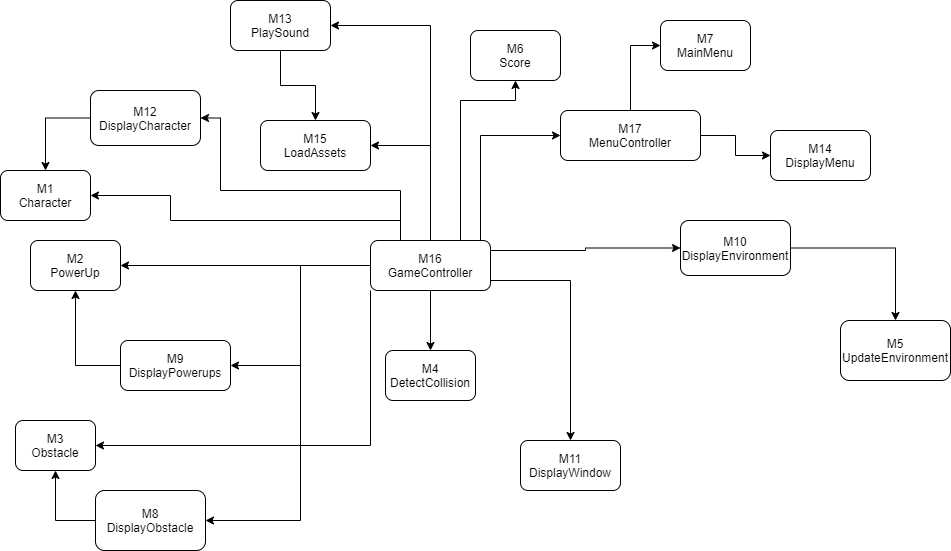
\includegraphics[width=1\textwidth]{Module Hiearchy.png}
\caption{Use hierarchy among modules \textcolor{red}{(Rev0)}}
\label{FigUH}
\end{figure}
\begin{figure}[H]
\centering
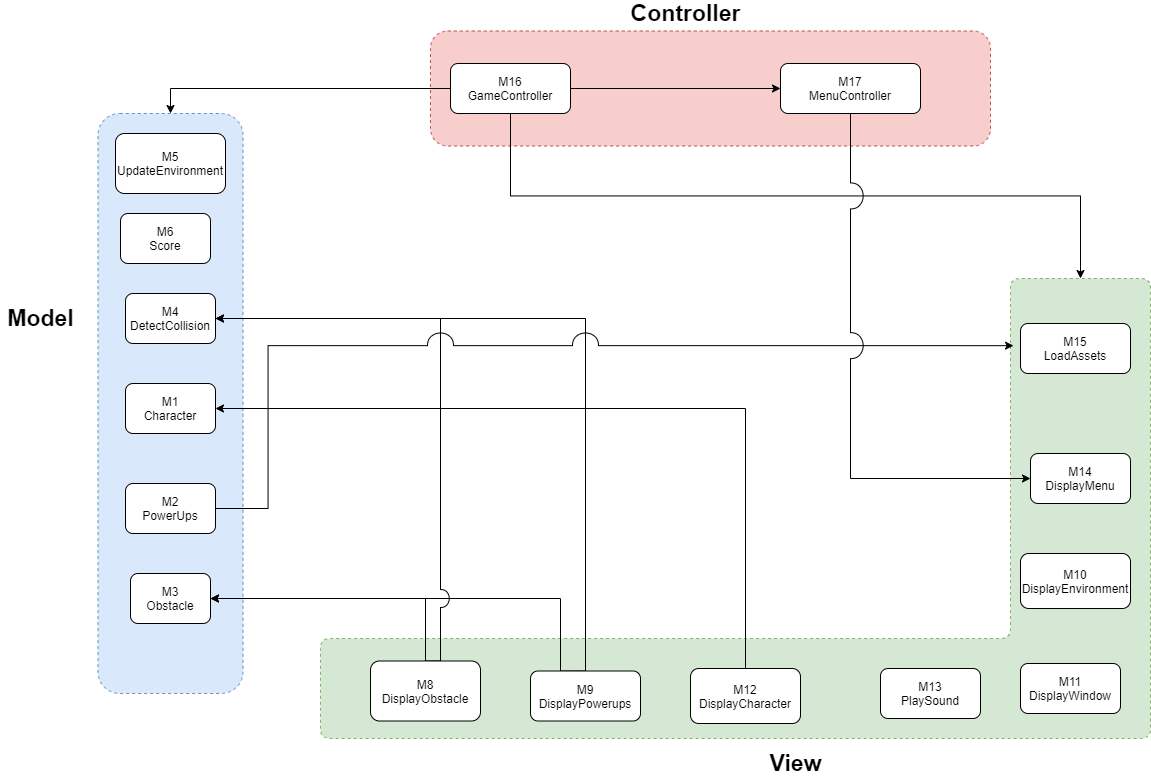
\includegraphics[width=1\textwidth]{Module Hiearchy_Rev1.png}
\caption{\textcolor{red}{Use hierarchy among modules (Rev1) }}
\label{FigUH}
\end{figure}

%\section*{References}

\bibliographystyle {plainnat}
\bibliography {MG}

\end{document}